%\documentclass{article}
%\usepackage{graphicx,subfigure}
%\begin{document}

\begin{figure}[!h]
  \centering
  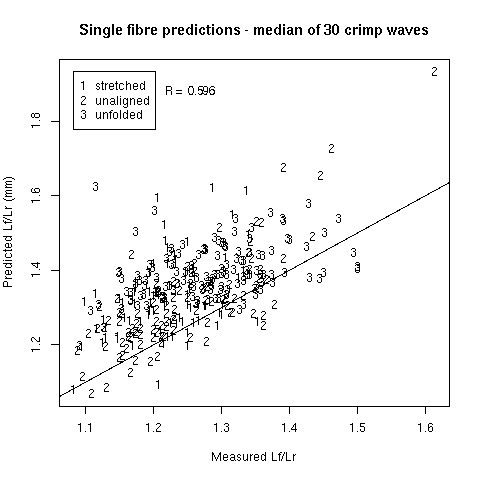
\includegraphics[width=1.1\textwidth]{figpredlftolrfibre.png}
% original is 15fibrepredlftolrmedian.png
  \caption{Plot of measured fibre stretched length to relaxed length ratio against predicted mean fibre stretched length to relaxed length ratio for 315 individual fibres with predictions based on measurement of wavelength and amplitude by the SF technique, and the ratio calculated using relaxed fibre length instead of staple length. Fibre lengths for the unfolded crimp type wools were adjusted for the effect of twist at the points of inflection using $H = 0.5 * amplitude$ and $R = 0.10 mm$ in the prediction equations }
  \label{fig:predlftolrfibre}
\end{figure}

%\end{document}

